\section*{Question 3}
In order to introduce while loops as a \texttt{statememt} of the while language, we again need to create a new java class for the abstract syntax. This class is inspired by the \texttt{IfStatement} class, and the main content can be seen in the code snippet below:

\begin{lstlisting}
private BoolExpr condition;
private Statement doBranch;
public WhileStatement(BoolExpr condition, Statement doBranch) {
	this.condition = condition;
	this.doBranch = doBranch;
}

@Override
public void evaluate(Environment env) throws VariableNotDefinedException {
	while (condition.evaluate(env)) {
		doBranch.evaluate(env);	
	} 
}
\end{lstlisting}

As seen, the class takes two parameters in the constructor: the condition and the expression to execute, as long as the condition is true. This is converted into a standard while loop in java when evaluated in the \texttt{evaluate} method. The \texttt{base\_statement} rule also contains the while statement, as seen below:

\begin{lstlisting}
base_statement returns [Statement value]
  : ID ':=' e=arith_expr    { $value = new AssignStatement($ID.getText(), e); }
  | 'if' c=bool_expr 'then' s1=base_statement 'else' s2=base_statement  { $value = new IfStatement(c,s1,s2); }

  //NEW
  | 'while' c=bool_expr 'do' s1=base_statement  { $value = new WhileStatement(c, s1); }

  | '{' s=statement '}' { $value = s; }
;
\end{lstlisting}

The new rule can be seen in use, in figure \ref{fig:Q3ex}

\begin{figure}[H]
    \centering
    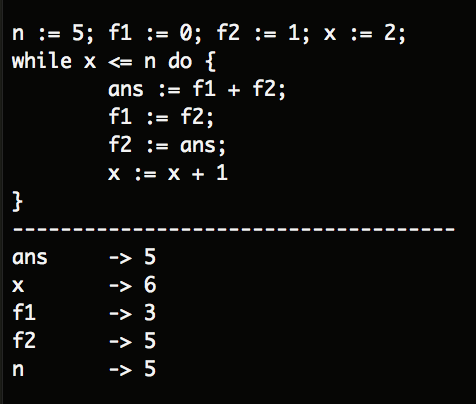
\includegraphics[width=0.4\textwidth]{fig/Q3example}
    \caption{While loop example with correct answer of ans = 5 (5'th fibonacci number).}
    \label{fig:Q3ex}
\end{figure}